\documentclass[gmd]{copernicus}
% ,manuscript

%% \usepackage commands included in the copernicus.cls:
%\usepackage[german, english]{babel}
%\usepackage{tabularx}
%\usepackage{cancel}
%\usepackage{multirow}
%\usepackage{supertabular}
%\usepackage{algorithmic}
%\usepackage{algorithm}
%\usepackage{amsthm}
%\usepackage{float}
%\usepackage{subfig}
%\usepackage{rotating}


\usepackage{graphicx}
\usepackage{amssymb,amsmath,epsfig,color} 
\usepackage{rotating} 
\usepackage{wasysym}   
\usepackage{natbib,url} 
\usepackage{listings}
\lstset{ basicstyle=\ttfamily, columns=fullflexible, frame=single, }
\usepackage[export]{adjustbox} 
\lstdefinelanguage{json}{morestring=[b]", morestring=[d]'}

\usepackage{algorithm,mdframed}
\usepackage{algorithmic}


\begin{document}

\title{Concepts and capabilities of the Instructed Glacier Model (3.X.X)}


\Author[1]{Guillaume}{Jouvet} 
\Author[1]{Brandon}{Finley}
\Author[]{other}{authors}



\affil[1]{Université de Lausanne, Switzerland}

\runningtitle{IGM 3.0.0}

\runningauthor{IGM authors}

\received{}
\pubdiscuss{} %% only important for two-stage journals
\revised{}
\accepted{}
\published{}

%% These dates will be inserted by Copernicus Publications during the typesetting process.

\firstpage{1}

\maketitle

{\textbf{\textcolor{red}{This document refer to IGM v3.X.X. Check the tag v.2.2.2 of this repo for the older release v.2.2.2. }}} \\

\textit{{This working document intends to be submitted for publication in a model development journal. It is opened for contributions. Contributions typically include the development of modules, or the performing and reporting of numerical experiments that assess the capabilities of IGM. All contributors will be listed as co-authors of the final paper. To date, direct contributors are (listed alphabetically): Samuel Cook, Guillaume Cordonnier, Andreas Henz, Oskar Herrmann, Tancrède Leger, Fabien Maussion, Jürgen Mey, Dirk Scherler, Claire-Mathile Stücki, Ethan Welty. Contact G. Jouvet if you wish to contribute.}} \\

\begin{abstract}
We present the concept and capabilities of the Instructed Glacier Model (IGM, https://github.com/jouvetg/igm), a Python-based modeling tool designed for efficiently simulating glacier evolution across various scales. For that purpose, IGM couples high-order ice thermomechanics, climate-driven surface mass balance, and mass conservation. Within IGM, the update of all physical model components involves a series of fully-rasterized mathematical operations performed by the TensorFlow library. This choice results in high parallelization capabilities, particularly beneficial when executed on GPU hardware. The specificity of IGM is that it models ice flow with a physics-informed convolutional neural network trained from high-order ice flow physics. Beside rasterizing its solving, this approach advantagously comes with automatic differentiation, which strongly facilitates model inversion (or data assimilation). IGM's design is focused on i) accessibility to a large community of glaciologists, ii) modularity to facilitate community development and customization, iii) reproducibility and large ensemble simulation capability, and iv) compatibility with OGGM for data access. We present IGM's physical and numerical models, the implementation and usage with a comprehensive workflow enabling the quick modeling of any mountain glacier based on the RGI ID. An ensemble of benchmark simulations demonstrates the physical and computational capabilities of IGM to simulate the evolution of paleo and contemporary glaciers.
\end{abstract}

\copyrightstatement{TEXT} %% This section is optional and can be used for copyright transfers.


\introduction  %% \introduction[modified heading if necessary]


Glacier evolution models permit to reconstruct the historical behavior of glaciers and their relationship with past climates. Additionally, they are indispensable 
for predicting how glaciers will evolve in the future and the consequent rise in sea levels due to climate warming \citep{pattyn2018paradigm}. Over the last two decades, the glaciological community has dedicated substantial efforts to the development of these models \citep[See the review by][]{zekollari2022ice}. These models are designed to encompass a wide range of pertinent physical processes, including ice flow, thermodynamics, subglacial hydrology, and their intricate interactions with various factors such as atmospheric conditions (e.g., climate-driven surface mass balance), the Earth's lithosphere, and the ocean (e.g., iceberg calving or subaquatic melting). Prominent examples of such models include Full-Stokes such as Elmer/Ice \citep{Gagliardini.etal.2013} for a generic usage, high-order such that PISM \citep{Winkelmann2011}, CISM \citep{lipscomb2019description}, ISSM \citep{larour2012continental}, which are popular in the ice sheet modelling community,
and SIA-based such as OGGM \citep{maussion2019open} or PyGEM \citep{rounce2020glacier}, which were designed for global glacier modelling. However, the increasing complexity of models (based on high-order mechanics) as well as the significant increase of observational data to assimilate comes with rising computational burdens. Parallel computing as well as automatic differentiation sounds like a promising way to overcome these limitations.


\textcolor{red}{[GJ: UPT WITH MOST RECENT LITTERATURE, ESP PI-ML]}
In recent years, there has been a growing interest in employing Graphics Processing Units (GPUs) to tackle the computational bootleneck in ice flow modeling. GPUs are equipped with a larger number of cores, albeit at slower speeds compared to Central Processing Units (CPUs). GPUs have the potential of overcoming previously mentioned limitations in modeling ice flow and achieve substantial speed improvements \citep{rass2020modelling}. Effectively harnessing the power of GPUs hinges on the implementation of numerical methods that can be subdivided into numerous parallel tasks, a particularly challenging endeavor when dealing with the viscous behavior of ice and the underlying diffusion equations governing its motion. A natural approach involves the explicit time integration of the Shallow Ice Approximation (SIA) \citep{vivsnjevic2020climatic}, the Second Order SIA \citep{braedstrup2014ice}, or the Stokes model \citep{rass2020modelling}. While programming on GPU was a relative complex task in the past, the emergence of libraries such as TensorFlow and PyTorch in the popular Python language opens new opportunities for the development of efficient glacier ice flow model at relatively limited technical level.
 
Capitalizing on recent library for efficient computation on GPU and machine learning techniques, we outline the concept and demonstrate the capability of a Python-based glacier evolution model -- the Instructed Glacier Model (IGM) -- originally introduced by \citet{jouvet2022deep} -- which couples ice thermomechanics, surface mass balance, and mass conservation. The specificity of IGM is that all physical model components are updated using relatively short sequence of operations on horizontal raster grids, making the workflow efficiently parrallelizable on GPU. Model components that do not involve any horizontal diffusion (such as the surface mass balance or the Enthalpy models) are easily solved raster-wise. In contrast, we use a Convolutional Neural Network (CNN) trained to satisfy high-order ice flow physics \citep{jouvet2023ice} to ensure the parrallization of this task. Using a CNN to model the ice flow has an other major advantage for data assimilation as embedded automatic differentiation tools permits to access all their derivatives, and therefore to perform model inversion \citep{jouvet2023inversion}. Lastly, IGM is implemented in the widely-used programming language, Python, to make it accessible to a large community of glaciologists and leverage the numerous Python libraries such as TensorFlow for efficient computation on GPU, OGGM for data access, and Hydra for parameter handling. Additionally, we have designed IGM in a modular fashion to facilitate community development and user customization of the model.

This paper is organized as follows. First, we describe the physical and numerical models and implemented in IGM. Then, we describe the implementation and the usage.
Last, we demonstrate its capabilities by presenting some examples of applications.
  
\section{Model}   

In the following, we use the notations $b(x,y)$, $s(x,y,t)$, and $h(x,y,t)$ to represent the glacier bedrock, upper surface, and ice thickness (Fig. \ref{notations}). Here, $(x,y)$ and $t$ denote horizontal coordinates, and the time. We also introduce ${\bf u}(x,y,z,t) = (u_x,u_y,u_z)$ as the 3D velocity field of the ice, and $T(x, y, z, t)$ and $\omega(x,y,z,t)$ to represent temperature and water content, respectively. 

\begin{figure*}[!h]
\begin{center} 
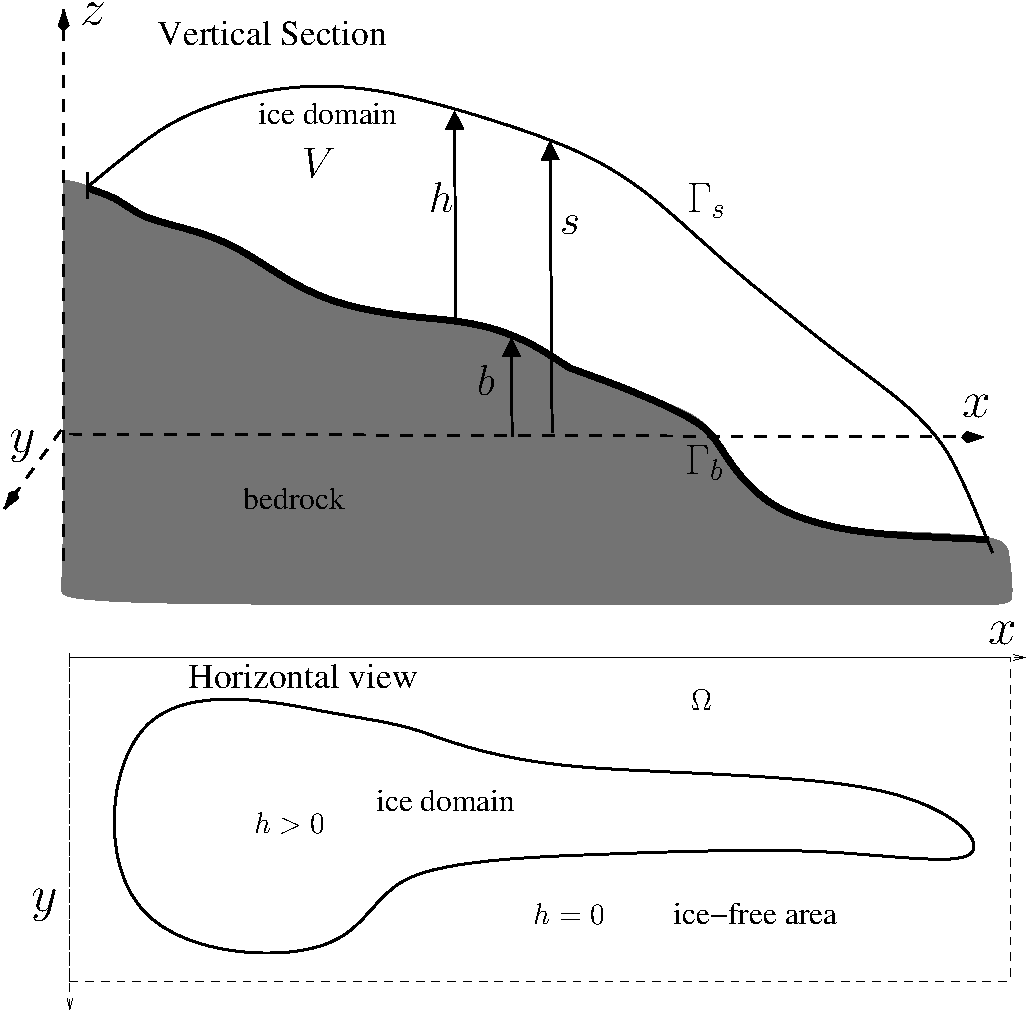
\includegraphics[width=0.48\textwidth]{fig/scheme.pdf}   
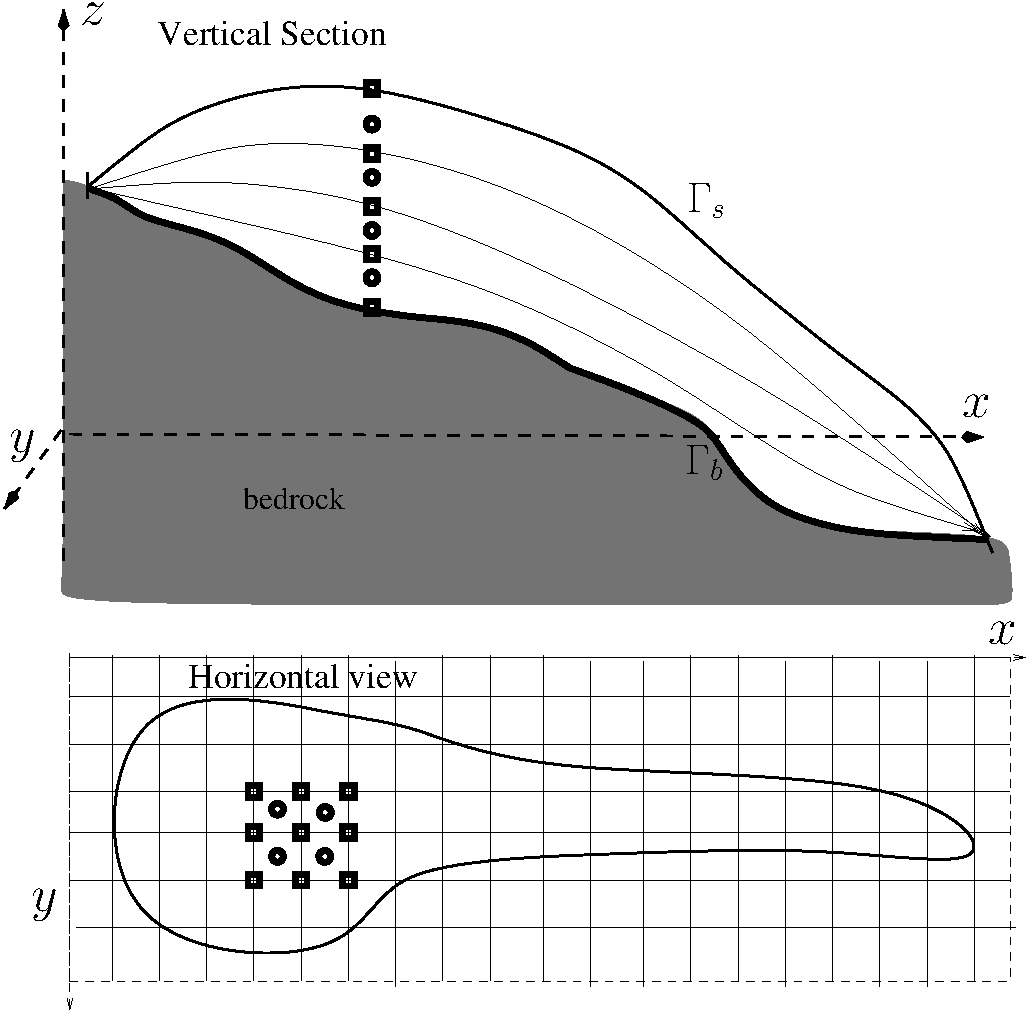
\includegraphics[width=0.48\textwidth]{fig/scheme_dis.pdf} 
\end{center}
\caption{Cross-section and horizontal view of a glacier with notations (left panel) and its spatial discretization (right panel), which is obtained using a regular horizontal grid and by subdividing the glacier into a pile of layers. All modelled variables (e.g. ice thickness) are computed at the corners of each cell of the 2D horizontal grid (materialised with squares) except the ice flow velocities, which are computed on the 3D corresponding grid. In contrast, the strain rate is computed on the staggered grid at the centre of each cells and layers (vizualized with circles). \label{notations}}
\end{figure*}

\subsection{Forward physical modelling}

Here, we describe all the physical models that are included in IGM and govern the evolution of the above-defined variables (Fig. \ref{notations}). Note that some model components (e.g., the Enthalpy) may be ignored for simplicity, while some others (e.g., the mass conservation) are always included.

\subsubsection{Surface mass balance}
\label{phys_smb}

IGM comes with several Surface Mass Balance (SMB) models, which compute the mass balance at the glacier surface. The SMB is the sum of the surface accumulation and ablation over one year. The SMB is computed at each grid cell of the horizontal domain and is used to update the ice thickness (Section \ref{phys_mass_conservation}). IGM includes three SMB models:

\begin{itemize}
\item The \texttt{smb\_simple} one implements a classical linar relation between Equilibrium Line Altitude (ELA) and altitude:
\begin{align}
SMB(z) & = \min(\beta_{acc} (z-z_{ELA}),m_{acc})\quad\textrm{if}\;z>z_{ELA}, \label{smb1} \\
SMB(z) & = \beta_{abl} (z-z_{ELA})\quad\textrm{else}, \label{smb2} 
\end{align}
where $z_{ELA}$ is the ELA, $\beta_{abl}$ and $\beta_{acc}$ are ablation and accumulation gradients, and $m_{acc}$ is the maximum SMB.
 
\item The \texttt{smb\_oggm} implements a combined accumulation / Positive Degree-Day (PDD) \citep{hock2003} to calculate the SMB based on seasonal temperature and precipitation fields. In this model, surface accumulation equals solid precipitation when the temperature is below a threshold (usually $0^{\circ}$C) and decreases linearly to zero in a transition zone. Conversely, surface ablation is computed in proportion to the number of PDDs. Given monthly temperature $T_i$ and precipitation $P_i$ spatial fields, the yearly SMB at elevation $z$ is then computed with 
\begin{align}
SMB = \frac{\rho_w}{\rho_i} \sum_{i=1}^{12} \left( P_i^{sol} - d_f \max \{ T_i - T_{melt}, 0 \} \right),
\label{smb3} 
\end{align}
where $P_i^{sol}$ is the monthly solid precipitation, $T_i$ is the monthly temperature and $T_{melt}$ is the air temperature above which ice melt is assumed to occur, $d_f$ is the melt factor, and $\frac{\rho_w}{\rho_i}$ is the ratio between water and ice density.

\item The \texttt{smb\_accme} implements an accumulation scheme similar to the \texttt{smb\_oggm}, but a more elaborate PDD model \citep[cf.][]{hock2003}: The surface ablation is computed proportionally to the number of PDD, however, we track the snow layer depth, and different PDD proportionality factors or ice. The PDD integral is numerically approximated using week-long sub-intervals based on \citet{calov2005}. Also, a fraction of the melt is assumed to refreeze.

\end{itemize}
 
\subsubsection{Ice flow}
\label{phys_ice_dynamics}
 
The momentum conservation equation (assuming negligible inertial terms) and the incompressibility condition are expressed as follows:
\begin{align}
- \nabla \cdot \sigma  & =  \rho  {\bf g},  \label{eq_conservation}  \\
\nabla \cdot {\bf u}  & = 0,                   \label{eq_incomp} 
\end{align}  
where $\sigma$ is the Cauchy stress tensor, ${\bf g}= (0,0,-g)$, $g$ is the gravitational constant. Let $\tau$ be the deviatoric stress tensor defined by 
\begin{align}
\sigma = \tau  -  p I , \label{eq_dev}  
\end{align}  
where $I$ is the identity tensor, $p$ is the pressure field, with the requirement that ${\rm tr} (\tau) = 0 $ so that $p = -(1/3) {\rm tr} (\sigma)$. Glen's flow law \citep{Glen1953}, which characterizes the mechanical behavior of ice, can be formulated as the following nonlinear relationship:
\begin{align} 
\tau & = 2 \mu {D} ({\bf u}), \label{eq_tau} 
\end{align}  
where ${D} ({\bf u})$ denotes the strain rate tensor defined by 
\begin{align} 
{D} ({\bf u}) = \frac12 ( \nabla {\bf u} +  \nabla {\bf u}^T ),
\label{def_varepsilon}  
\end{align} 
$\mu$ is the viscosity defined by 
\begin{align}  
\mu & = \frac12  A^{-\frac{1}{n}} | D ({\bf u}) |^{\frac{1}{n}-1},
\label{eq_mu}  
\end{align} 
where $ |Y|  := \sqrt{(Y : Y) / 2 }$ denotes the norm associated with the scalar product $(\; : \;)$ (the sum of the element-wise product), $A=A(x,y,z,t)$ is the Arrhenius factor and $n>1$ is the Glen's exponent. Note that $A$ depends on the temperature of the ice \citep{Paterson1994} \textit{via} Glen-Paterson-Budd-Lliboutry-Duval law:
\begin{align}
A(T,\omega)= A_c(T)(1+181.25 \omega), \label{defA}
\end{align}
where $A_c(T)$ is given by the Paterson-Budd law:
\begin{align}
A_c(T)= A \exp{ ( -Q / (R \, T_{pa}) )},
\end{align}
where $A$ and $Q$ have different values below and above a threshold temperature:
\begin{align}
A & = 3.985 \times 10^{-13} \, s^{-1} Pa^{-3}, & \textrm{ if } T <263.15 \, K \label{A1} \\
A & = 1.916 \times 10^3 \, s^{-1} Pa^{-3}, & \textrm{else.} \label{A2} 
\end{align}
and
\begin{align}
Q & =  60 \; {\rm kJ mol}^{-1}, & \textrm{ if } T <263.15 \, K \\
Q & = 139 \; {\rm kJ mol}^{-1}, & \textrm{else.}
\end{align}
We may ignore temperature dependence of $A$ for instance in the case the Enthalpy (Section \ref{phys_enthalpy}) is not modelled.
 
Equations \eqref{eq_conservation} to \eqref{eq_mu} describe a Stokes problem in which the unknowns are the 3D velocity field ${\bf u}$ and the pressure field $p$. To simplify the problem, we make the "hydrostatic assumption" as described by  \citep{Blatter1995} and neglect second-order terms in the aspect ratio of the ice domain (thickness versus length) within the strain rate tensor $D({\bf u})$. By doing so and invoking the incompressibility equation, both the vertical velocity components $u_z$ and the pressure $p$ are eliminated from the momentum conservation equation. The resulting model, commonly referred to as the Blatter-Pattyn model \citep{Blatter1995}, conveniently transforms into a 3D nonlinear elliptic equation solely for the horizontal velocity components. This modification makes it easier to solve compared to the original Stokes model.

The boundary conditions that supplement \eqref{eq_conservation}, \eqref{eq_incomp} are the following. Stress free force applies to the ice-air interface,
\begin{equation}
\sigma \cdot {\bf n} = 0, \quad p = 0,  \label{BC_FS}
\end{equation}
where ${\bf n}$
is an outer normal vector along the surface. Along the lower surface interface, the nonlinear Weertman friction condition \citep[e.g.,][]{SchoofHewitt2013} relates the basal shear stress $\tau_b$ to the sliding velocity ${\bf u}_b$ as follows:
\begin{align}
{\bf u} \cdot {\bf n} &= 0,  \label{BC_slip1} \\ 
\tau_b & = -  c |{\bf u}_b|^{m-1} {\bf u}_b, \label{BC_slip2a}
\end{align} 
where $m>0$, $c=c(x,y) > 0$, and ${\bf n}$ is the outward normal unit vector to the bedrock.

The sliding coefficient $c$ in \eqref{BC_slip2a} is defined with the Mohr-Coulomb law \citep{Cuffey.2010}, that involves the effective pressure in the till $N_{till}$ (Section \ref{phys_subglacial_hydrology}):
\begin{align}
c  = \tau_c u_{th}^{-m} & = N_{till} \tan(\phi) u_{th}^{-m}, 
\label{sliding_param}
\end{align}
where $\phi$ is the till friction angle, and $u_{th}$ is a parameter homegenous to  ice velocity following \citet{pism-user-manual}. In the case the Enthalpy (Section \ref{phys_enthalpy}) and the subglacial hydrology (Section \ref{phys_subglacial_hydrology}) are not modelled, we may simply prescribe a constant sliding coefficient $c$, or get its spatial distribution by inverse modelling (Section \ref{inv_model}).

Conditions on the top surface are free-stress:
\begin{align}
 A^{-\frac{1}{n}} | D({\bf u}) |^{\frac{1}{n}-1} D({\bf u}) \cdot {\bf n} =  0.
\label{BC_SSA0}
\end{align}  

\textcolor{red}{[GJ:PROVIDE THE DERIVATION BLATTER/ENERGY IN APPENDIX]}
Following \citet{jouvet2016mechanical}, the Blatter-Pattyn problem is rewritten as an energy-minimization problem associated with the functional:
\begin{align}
\mathcal{J} ({\bf v}) & =
\int_{V} 2 \frac{A^{-\frac{1}{n}}}{1+\frac{1}{n}} |  D ({\bf v}) |^{1+\frac{1}{n}}  dV  
+  \int_{\Gamma_b} \frac{c}{1+m}  |{\bf v}|^{1+m}_M   dS  \nonumber \\
& +  \rho g \int_{V} ( \nabla s \cdot {\bf v} ) dV,
\label{functional}
\end{align}
where $V$, and $\Gamma_b$ denote the ice volume and bedrock interface.

Note that while Blatter-Pattyn model permits to obtain the horizontal components of the ice velocity $(u_x,u_y)$, the third and vertical component $u_z$ can be obtained by integrating vertically the imcompressibility condition \eqref{eq_incomp}.

\subsubsection{Mass conservation}
\label{phys_mass_conservation}

The evolution of ice thickness, denoted as $h(x, y, t)$, starting from an initial glacier shape, is governed by mass conservation, which connects elevation change, ice dynamics and SMB (Fig. \ref{notations}) through:
\begin{equation}
\frac{\partial h}{\partial t} + \nabla \cdot \left( \bar{\bf u} h \right) = {\rm SMB},
\label{conservationeq}
\end{equation}
where symbol $\nabla \cdot$ represents the divergence operator for the horizontal variables $(x, y)$, $\bar{\bf u} = (\bar{u}, \bar{v})$ denotes the vertically-averaged horizontal ice velocity field, while ${\rm SMB}$ represents the surface mass balance.
 
\subsubsection{Ice enthalpy}
\label{phys_enthalpy}

In this section, we model ice enthalpy following \citet{aschwanden2012enthalpy}. This approach enables us to simultaneously model ice temperature and water content when the temperature reaches the pressure melting point, thereby conserving energy. Ice enthalpy influences the dynamical model in two ways: variations in temperature and water content lead to ice softening or hardening (Eq. \eqref{defA}), while enthalpy affects basal sliding conditions throught basal till water layer (Eq. \eqref{sliding_param}). The enthalpy, denoted as $E$, is a variable defined throughout the ice and is a function of both temperature, $T$, and water content, $\omega$:
\begin{align}
\label{def_enth}
E(T, \omega,p) = 
\left\{
\begin{array}{ll}
c_i (T- T_{\rm ref}), & {\rm  if } \; T < T_{\rm pmp} , \\ 
E_{\rm pmp} + L \omega, &  
{\rm if } \;  T = T_{\rm pmp},\; 0 \le \omega,
\end{array} 
\right.  
\end{align}
where $c_i$ is the heat capacity, $T_{ref}$ is a reference temperature, and $L$ is the latent heat of fusion. Additionally the temperature $T_{\rm pmp}$ and enthalpy $E_{\rm pmp}$ at pressure-melting point of ice are defined by   
\begin{align}
T_{\rm pmp} & = T_0 - \beta p, \label{defTpmp} \\
E_{\rm pmp} & = c_i (T_{\rm pmp}(p) - T_{\rm ref}), \label{defEpmp}
\end{align}  
where $T_0 = 273.15$ K is the melting temperature at standard pressure, and $\beta = 7.9 \times 10^{-8}$ K Pa$^{-1}$ is the Clausius-Clapeyron constant. 

According to the definition of enthalpy provided above, we have two possible modes: i) When the ice is cold, meaning it is below the melting point, the enthalpy is simply proportional to the temperature minus a reference temperature. ii) When the ice is temperate, the enthalpy continues to increase. In this case,  the additional component $L \omega$ accounts for the creation of water content through energy transfer. Therefore, one can infer the value of enthalpy, denoted as $E$, from both temperature, $T$, and water content, $\omega$, and \textit{vice-versa}.

The melting point temperature at pressure is adjusted for hydrostatic pressure $p = \rho g d$ using the following equation:
\begin{equation}
\label{Tpmp}
T_{pmp} = T_{0} - \beta \rho g d, 
\end{equation}
where $d$ represents the depth. Therefore, the "pressure-adjusted" temperature, 
denoted as $T_{pa}$, is defined as the temperature with a shift such that its 
melting point temperature reference is always zero:
$$ T_{pa} = T + \beta \rho g z. $$

The enthalpy model consists of the following advection-diffusion equation,
with horizontal diffusion being neglected:

\begin{align}
& \rho_i \left( \frac{\partial E}{ \partial t}
+ u_x \frac{\partial E}{ \partial x}
+ u_y \frac{\partial E}{ \partial y} 
+ u_z \frac{\partial E}{ \partial z} 
\right) 
 - \frac{\partial }{\partial z} \left(
K_{c,t} \frac{\partial E}{ \partial z} \right) \label{enth1} \\
& = \phi - \rho_w L D_w(\omega), \label{enth2} 
\end{align}

where $\rho_i$ is the ice density, $K_{c,t}$ equals 
$K_c = k_i/c_i$ if the ice is cold ($E<E_{pmp}$) or $K_t = \epsilon k_i/c_i$ otherwise. 
Using Glen's flow law (Eq. \eqref{eq_tau}), the strain heating $\phi$ is defined by 
\begin{equation}
\label{def_phi}
\phi = D({\bf U}) \tau = A^{-1/n} | D({\bf u}) |^{1+1/n}.
\end{equation}
The last source term $- \rho_w L D_w(\omega)$ in \eqref{enth2} permits to remove the water 
in temperate ice, $D_w(\omega)$ being a drainage function \citep{aschwanden2012enthalpy}.

At the top ice surface, the enthalpy equation is constrained by the surface temperature 
(or equivalently, the enthalpy) provided by the climate forcing, which is enforced as a 
Dirichlet condition.
At the glacier bed, there are multiple boundary conditions for the enthalpy equation
\citep{aschwanden2012enthalpy,wang2020two}:
\begin{itemize}
\item cold base and dry: $K_{c} \frac{\partial E}{ \partial z} = Q_{\rm geo} + Q_{\rm fh}$
if $E_b<E_{\rm pmp}$ and $W_{till} = 0$, 
\item cold base and wet: $ E_b = E_{\rm pmp} $ if $E_b<E_{\rm pmp}$ and $W_{till} > 0$,
\item temperate base and cold ice: $ E_b = E_{\rm pmp} $ if $E_b \ge E_{\rm pmp}$ and $W_{till}> 0$,
zero temperate basal layer,
\item temperate base, temperate ice: $ K_{t} \frac{\partial E}{ \partial z} = 0$ 
if $E_b \ge E_{\rm pmp}$ and $W_{till} > 0$, non-zero temperate basal layer,
\end{itemize}
where $Q_{\rm geo}$ and $Q_{\rm fh}$ are the geothermal heat flux, and the frictional heat flux, 
respectively. Using Weertmann law \eqref{BC_slip2a}, the latter is computed as follows:
\begin{equation}
Q_{\rm fh} = \tau_b \cdot {\bf u}_b = c | {\bf u}_b |^{m+1}. \label{def_Q}
\end{equation}
When the temperature hits the pressure-melting point at the glacier bed 
(i.e. $E \ge E_{\rm pmp}$), the basal melt rate is calculated via the following equation:
\begin{equation}
m_b = \frac{1}{\rho_i L} (Q_{fr}+Q_{geo} - K_{t,c} \frac{\partial E}{ \partial z}). 
\label{basal_melt_rate}
\end{equation}
The basal melt rate is further increased to account for the drainage of the water 
content generated throughout the entire column (last term of Eq. \eqref{enth2}).

\subsubsection{Subglacial hydrology}
\label{phys_subglacial_hydrology}

Following \citet{Bueler2015}, the basal water thickness in the till $W_{till}$ 
is computed from the basal melt rate as follows:
\begin{equation}
\frac{\partial W_{till} }{ \partial z} = \frac{m_b}{\rho_w} - C_{dr},
\label{W_till}
\end{equation}
where $C_{dr}$ is a simple drainage parameter. The till is assumed to be saturated 
when it reaches the value $W_{till}^{max} = 2$ m, therefore, the till water thickness 
is capped to this value. The effective thickness of water within the till $N_{till}$ 
is computed from the saturation ratio $s= W_{till} / W_{till}^{max}$ by the formula
\citep{Bueler2015}:
\begin{equation}
N_{till} = \min \left\{ p, N_0 \left( \frac{\delta P}{N_0} \right)^s 10^{(e_0/C_c)(1-s)} \right\},
\end{equation}
where $p$ is the ice overburden pressure and the remaining parameters are constant. 
 
\subsubsection{Lagrangian modelling}

While IGM's models are formulated in a Eulerian framework, IGM also includes a Lagrangian module to track the trajectory of (physical or virtual) particles advected by the ice flow. Doing so is particularly useful for studying the evolution of tracers within the ice such as debris, morainic material, or simply to track the age and properties of ice. The trajectory 
of the particle passing $\bar{\bf x}$ at time $\bar{t}$ on the
time interval $I_{\bar{t}}$ solves the ordinary differential equation:
\begin{equation}
 \label{pathline}
\left\{
\begin{array}{ll}
\frac{d \bf x}{dt}(t)  & = {\bf u} ( {\bf x}(t), t),  \qquad \text{on} \; I_{\bar{t}}, \\
{\bf x} (\bar{t})  & = \bar{\bf x}.
\end{array} 
\right.
\end{equation} 

\subsection{Forward numerical modelling}

In IGM, the horizontal modeled domain is assumed to be a rectangle. IGM deals with rastered data defined on a regular grid of dimensions $N_x \times N_y$ and uniform spacing along both the $x$ and $y$ axes (Fig. \ref{notations}, right panel). Key variables such as ice thickness $h$, surface topography $s$, or sliding coefficient $c$ are defined on this grid. It is important to note that our choice of a structured grid, rather than any other type of more complex discretization, is crucial for representing variables as 2D arrays. This structure allows us to employ Convolutional Neural Networks (CNN) for emulating the mechanics of ice flow (Section \ref{module_iceflow}). On the other hand, the discretization of ice thickness occurs vertically using a fixed number of points denoted as $N_z$ (Fig. \ref{notations}, left panel). These layers can be distributed in a non-uniform manner, e.g. to ensure finer discretization near the ice-bedrock interface, where the steepest gradients are expected, and coarser near the ice-surface interface following the strategy proposed in the Parallel Ice Sheet Model \citep[PISM,][]{pism-user-manual}. Note that in the special case of $Nz=2$, the ice velocity profile from the bottom to the top of the ice is assumed to vary polynomially following the Shallow Ice Approximation (SIA) formula similarly to the approach proposed by \citet{dias2022new}. In the case of a single layer ($Nz=1$), the ice flow is assumed to be vertically uniform, and the ice flow model reduces to the Shallow Shelf Approximation (SSA).

IGM employs a time-advancing algorithm that permits to update SMB, iceflow,  possibility enthalpy, and ice thickness over time. For efficiency reason, the key is to perform all these updates raster-wise with the Tensorflow library, i.e. in parallel over all cells of the horizontal grid, however, making sure that these updates involve a relatively short sequence of operations: in $\mathcal{O}(\textrm{CNN's number of layers})$ for the ice flow, in $\mathcal{O}(\textrm{SMB time step})$ for the SMB, and in $\mathcal{O}(Nz)$ for the enthalpy.
%i) the ice flow is computed by using a CNN that performs grid-to-grid mapping with a relative short track of operations (the number of layers), ii) the SMB is computed applying a formula that applies on the entire grid, possibly sequential-wise (Section \ref{num_smb}), iii) the enthalpy is solved column-wise by finite difference, and iv) the mass conservation equation is solved using an explicit first-order upwind finite-volume scheme. 
For clarity and modularity, IGM separates these steps into distinct modules within the modeling framework.

\subsubsection{Surface mass balance}
\label{num_smb}

The SMB models presented in Section \ref{num_smb} are implemented in IGM applying formula \eqref{smb1}-\eqref{smb3} on the entire grid. Therefore the computation of the SMB is fully rasterized and can be computed in parallel on the GPU. Only the PDD model with tracking of the snow layer (\texttt{smb\_accmelt}, which applies different PDD parameters on snow and ice) needs to be computed sequentially in time, and can therefore not be parallelized. Its execution costs scales therefore linearly with the number of time steps used for the SMB and can therefore be considered as a bottleneck if small time steps are used (typically daily or weekly).
 
\subsubsection{Ice flow}
\label{num_iceflow}

\textcolor{red}{[TODO: ADD THE CASE $Nz=1,2$]}

Following \citet{jouvet2023ice}, the ice flow dynamics in 3D is modelled using a Physics-Informed Convolutional Neural Network (CNN). The CNN predicts horizontal ice flow $({\bf u}_H, {\bf v}_H)$ from input fields which includes ice thickness $h_H$, surface topography $s_H$, ice flow parameters $A_H$ and sliding coefficient $c_H$, and spatial grid resolution $H_H$ (Fig. \ref{mapping-illu}). The CNN is trained to minimize the energy \eqref{functional} associated with the Blatter-Pattyn ice flow model. The optimisation problem is solved using the Adam optimiser \citep{kingma2014adam} -- the derivatives of the energy with respect to the weights of the CNN being obtained from automatic differentiation.

This approach offers a GPU-accelerated alternative to traditional solvers, along with the ability to memorize previous solutions and take advantage of this for accuracy improvement \citep{jouvet2023ice}. In IGM, we initially load a pretrained iceflow emulator (to start with a good initial guess) provided with the IGM package, and  retrain it regularly within the time loop to maintain its accuracy. This frequent retraining permits the CNN to adapt to the new glacier geometries met during the glacier evolution. Note that the retraining costs are about 3 times more than a CNN evaluation (since it requires to pass over the CNN in the two directions), we strive to find a trade-off frequency: not too frequent to mitigate the costs, and not to rare to maintain the accuracy of the emulator. It should be stressed that the retraining task is memory consuming since it involves storing all the operations of the CNN. Therefore, the maximal size of the raster grid that can be used with IGM is limited by the available GPU memory, otherwise a more costly strategy should be used to retrain sequentially and patch-wise the CNN.

\begin{figure}[!ht]
\begin{center}
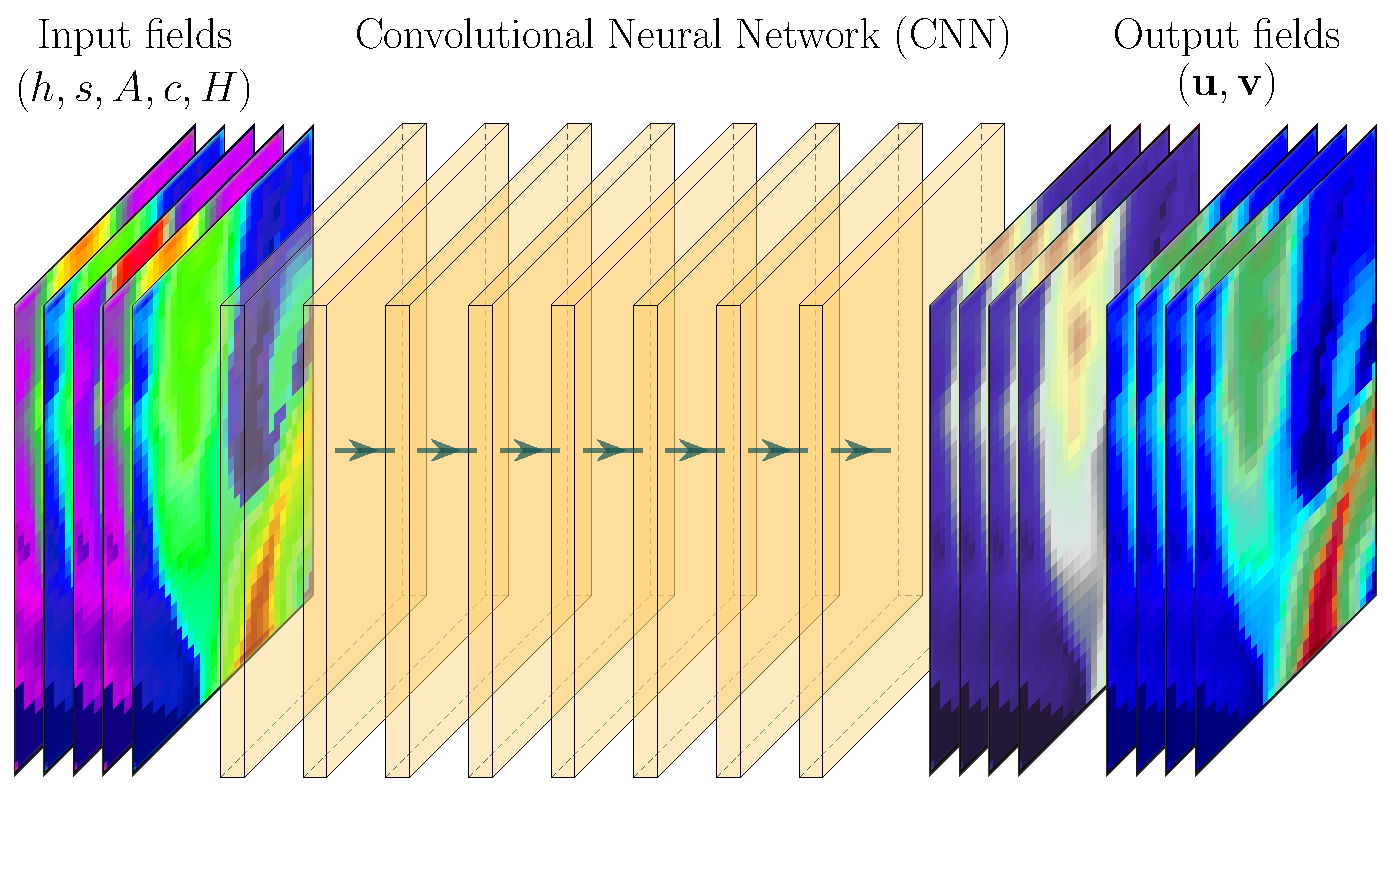
\includegraphics[width=0.48\textwidth]{fig/mapping-illu7.pdf}
\caption{\label{mapping-illu} Our iceflow emulator consists of a CNN that maps geometrical (thickness and surface topography), ice flow parameters (shearing and basal sliding), and spatial resolution inputs to the horizontal ice flow field in 3D.}
\end{center}
\end{figure}

Should we require the vertical ice flow component (as required by the Enthalpy or the particle tracking), its computation is achieved by integrating numerically the incompressibility condition \eqref{eq_incomp} over the vertical discretization layers (Fig. \ref{notations}, right pannel) from the bottom to the top of the ice.

\subsubsection{Mass conservation}
\label{num_mass_conservation}

Solving mass conservation equation \eqref{conservationeq} permits to update ice thickness from the iceflow and the SMB. This is done using an explicit first-order upwind finite-volume scheme on the 2D working grid. In this scheme, ice mass is permitted to move between adjacent cells where thickness and velocities are defined. This movement is determined by edge-defined fluxes, which are inferred from depth-averaged velocities and ice thickness in the upwind direction. The resulting scheme is both mass-conserving and parallelizable, thanks to its fully explicit nature. However, it is subject to a Courant-Friedrichs-Lewy (CFL) condition, yielding to an upper-bound on the time step. This condition guarantees that no more than the entire content of one cell is transferred to a neighboring cell within a single iteration.

The time step is therefore adjusted to remain below a designated maximum time step:
\begin{equation}
\Delta t \le  C \times \frac{ \Delta x }{ \Vert \bar{\bf u } \Vert_{L^{\infty}} },
\label{cfl}
\end{equation}
where $C<1$ and $\Delta x$ is the grid cell spacing. This CFL condition is key to ensure stability in the transport scheme for ice thickness evolution.

\subsubsection{Ice enthalpy and subglacial hydrology}
\label{num_enthalpy}

The 3D enthalpy field needs to be updated based on the mechanical state by solving the advection-diffusion equation \eqref{enth1}-\eqref{enth2}. This process includes applying the top and bottom boundary conditions described in Section \ref{phys_enthalpy}. To achieve this, the variable $E$ (and equivalently, $T$ and $\omega$) is defined on the same 3D structured grid than the ice flow field $\mathbf{u}$. \textcolor{red}{[TODO: CHANGE THIS, THE ENTALPY MUST HAVE ITS OWN GRID]}. Solving equations \eqref{enth1}-\eqref{enth2} is done in two steps through time splitting operators. First, an explicit first-order upwind finite-volume scheme is employed to solve the advective component in the horizontal direction, following a similar scheme as the one used in the mass conservation equation:
\begin{align}
 E^{n+\frac12}  = E^n - dt \left( u^n_x \frac{\partial E^n}{ \partial x} 
  + u^n_y \frac{\partial E^n}{ \partial y} \right),
\label{E_step1}
\end{align}
In a second time we solve the remaining advection-diffusion equation with respect to the vertical direction in an implicit manner:
\begin{align}
& \rho_i \left( \frac{E^{n+1}-E^{n+\frac12}}{ dt}
+ u_z \frac{\partial E^{n+1}}{ \partial z} \right) \\
& - \frac{\partial }{\partial z} \left(
K_{c,t} \frac{\partial E^{n+1}}{ \partial z} \right) 
 = \phi^n - \rho_w L D_w(\omega^{n+\frac12}).
\label{E_step2}
\end{align}

This is done by finite differences, where the advection term is approximated using an upwind method, while the diffusion term is approximated using a centered scheme. Once the top and bottom boundary conditions are incorporated, the discretization leads to solving $N_y \times N_x$ tridiagonal systems, each with 
a size equal to the number of layers $N_z$. Solving these tridiagonal systems is accomplished using the tridiagonal matrix algorithm (or Thomas algorithm). This algorithm requires approximately $3 \times N_z$ operations per column, translating to a total of $3 \times N_z \times N_y \times N_x$ operations in total. Tensorflow ensures  parallelism of operations between column-wise problems. Following solving the enthalpy equation, the process involves computing the basal melt rate using \eqref{basal_melt_rate}, updating it along with the enthalpy to account for water drainage along the ice column. This step also calculates the resulting water thickness from \eqref{W_till} and sliding coefficient from \eqref{sliding_param}.

In summary, assuming known enthalpy $E^n$, ice thickness geometry $h^{n+1}$, iceflow ${\bf u}^{n+1}$, vertical ice flow $u^{n+1}_z$, updating the enthalpy at time $t^{n+1}$ requires to perform the following sub-steps:
\begin{itemize}
\item Compute the mean surface temperature $T^n_s$ to enforce the upper surface Dirichlet boundary condition. This temperature is capped at 0$^{\circ}$C to maintain the temperature of ice below pressure-melting point.
\item Compute the vertical discretization with the new ice geometry $h^{n+1}$.
\item Compute the temperature $T_{pmp}^n$ and enthalpy $E_{pmp}^n$ at pressure melting point using \eqref{Tpmp}.
\item Compute the ice temperature $T^n$ from the enthalpy $E^n$ using \eqref{def_enth}.
\item Compute the Arrhenius factor $A(T^n)$ from temperature $T^n$ using \eqref{A1}-\eqref{A2}.
\item Compute the 3D strain heat $\phi^{n+1}$ from ice flow field ${\bf u}^{n+1}$ and Arrhenius factor $A(T^n)$ using \eqref{def_phi}.
\item Compute the 2D basal frictional heat $Q_{\rm fh}^{n+1}$, from basal velocity field ${\bf u}^{n+1}$ and sliding coefficient $c^n$ using \eqref{def_Q}.
\item Compute the surface enthalpy $E^n_s$ from the surface temperature $T^n_s$  using \eqref{def_enth}.
\item Compute the updated enthalpy $E^{n+\frac12}$ after solving one explicit step for the horizonal advection (Eq. \eqref{E_step1}).
\item Compute the updated enthalpy $E^{n+1}$ field solving the advection-diffusion equation (Eq. \eqref{E_step2}).
\item Compute the basal melt rate from \eqref{basal_melt_rate}.
\item Compute the water thickness in the till $W^{n+1}$ solving \eqref{W_till} explicity.
\item Compute the sliding parametrization $c^{n+1}$ using \eqref{sliding_param}.
\end{itemize}

\subsubsection{Particle tracking}
\label{num_particle_tracking}

A particle tracking routine calculates the time-space trajectory of virtual tracers that are advected by the ice flow. Thanks to TensorFlow's GPU implementation, a substantial number of particles can be efficiently computed in parallel. For that purpose, one uses a fourth order Runge-Kutta method to solve the ordinary differential equation \eqref{pathline} and obtain an approximation of the trajectory. Presently, there are two implementations available:
\begin{itemize}
\item In the \texttt{simple} implementation, particles are advected in the horizontal plane using the horizontal velocity field, with interpolation performed bilinearly. In the vertical direction, particles are tracked along the ice column, scaling their position between 0 and 1, where 0 represents the bed and 1 corresponds to the top surface. The evolution of the particles within the ice column over time is determined by the SMB: when the SMB is positive (indicating ice accumulation), the particles move deeper within the ice column, reducing their relative height. Conversely, when the SMB is negative (indicating ice ablation), the particles rise within the ice column, increasing their relative height. 
\item  In the \texttt{3d} implementation, the method advects particles from the the 3D ice flow velocity field. Unlike the \texttt{simple} method, one needs the vertical ice velocity component to be computed.
\end{itemize}
 
\subsection{Inverse modelling}
\label{inv_model} 
 
Inverse modelling (or data assimilation) serves to find optimal ice thickness, top ice surface, and ice flow parameters that align with observational data in a preliminary step. These observations can include surface ice speeds, ice thickness profiles, and top ice surface data. The goal is to find the fields that best explain the observed data while remaining consistent with the ice flow used in the forward modeling \citep{jouvet2023inversion,jouvet2023ice}. In the most general case, the corresponding optimization problem consists of finding spatially varying fields ($h$, $c$, $A$, $s$) that minimize the cost function
\begin{align}
\mathcal{J}(h,c,A,s) & =\mathcal{C}^u+\mathcal{C}^h+\mathcal{C}^s +\mathcal{C}^{d} \label{misfit} \\
&+\mathcal{R}^h+\mathcal{R}^{c}+\mathcal{R}^{A}+\mathcal{P}^h,  \nonumber
\end{align}
where $\mathcal{C}^u$ is the misfit between modeled ${\bf u}^{s}$ and observed 
${\bf u}^{s,obs}$ surface ice velocities 
\begin{align}
\mathcal{C}^u=\int_{\Omega}\frac{1}{2\sigma_u^2}\left|{\bf u}^{s,obs}-{\bf u}^{s}\right|^2,
\end{align} 
$\mathcal{C}^h$ is the misfit between modeled and observed $h^{obs}$ ice thickness available profiles:
\begin{align}
\mathcal{C}^h= \int_{\Omega}\frac{1}{2 \sigma_h^2}|h^{obs} -h |^2,
\end{align}
where $h^{obs}$ is a rasterized representation of ice thickness profiles
(the pixels with missing data are ignored in the above integral), and
$\mathcal{C}^s$ is the misfit between the modeled and observed $s^{obs}$ top ice surface:
\begin{align}
\mathcal{C}^s=\int_{\Omega}\frac{1}{2 \sigma_s^2}\left|s-s^{obs}\right|^2,
\end{align}
where $\mathcal{C}^{d}$ is a misfit term between the modeled and observed flux divergence $d^{obs}$:
\begin{align}
\mathcal{C}^{d}=\int_{\Omega}\frac{1}{2 \sigma_d^2}\left|\nabla \cdot (h {\bar{\bf u}})-d^{obs} \right|^2,
\end{align}
where $\mathcal{R}^h$ is a regularization term to enforce smoothness of $b=s-h$
and convexity of $h$:
\begin{align}
\mathcal{R}^h=\alpha_h\int_{h>0}\left(|\nabla b |^2 -\gamma h\right),
\end{align}
where $\mathcal{R}^{c}$ and $\mathcal{R}^{A}$ are regularization terms to enforce smooth sliding coefficient $c$ and Arrhenius factor $A$:
\begin{align}
\mathcal{R}^c=\alpha_c \int_{h>0}|\nabla c |^2, \qquad
\mathcal{R}^A=\alpha_A \int_{h>0}|\nabla A |^2,
\end{align}
where $\mathcal{P}^h$ is a penalty term to enforce nonnegative ice thickness, 
and zero thickness outside a given mask:
\begin{align}
\mathcal{P}^h=10^{10} \times \left(\int_{h<0} h^2+\int_{\mathcal{M}^{\rm ice-free}} h^2 \right).
\end{align}

Hereabove, we denote $\sigma_u$, $\sigma_h$, $\sigma_d$, $\sigma_s$ as the user-defined confidence levels (possibly spatially varying) errors of observations for ${\bf u}_s^{obs}$, $h_p^{obs}$, $d^{obs}$, and $s^{obs}$, respectively, and $\alpha_h, \gamma, \alpha_c, \alpha_A>0$ are fixed parameters.

Solving the optimization problem for the functional \eqref{misfit} is done using the Adam optimizer \citep{kingma2014adam}, which  leverages the automatic differentiation tools provided by the Tensorflow, and the description of the ice flow model as a neural network (Section \ref{module_iceflow}). In addition, the optimization is combined with retraining of the ice flow emulator to ensure that the ice flow model remains accurate throughout the optimization process. We refer to \citet{jouvet2023ice} for a detailed explanation of the methodology.
 
Note that the inverse modelling is designed to infer initial distributed sliding coefficient $c$ and/or the ice flow parameters $A$. It is therefore not designed to be combined with the enthalpy and subglacial hydrology models, which are computing prognostically these fields.
 
\section{Implementation and usage of IGM}

IGM is implemented in a Python package, which can be installed using pip directly from the source (\url{https://github.com/instructed-glacier-model/igm}) or from PyPi:
\begin{lstlisting}[language=bash,frame=single,numbers=none]
pip install igm-model
\end{lstlisting}

Once installed, we run IGM by calling the main script \texttt{igm\_run}, which accepts a wide range of parameters that are passed in a \texttt{params.yaml} file stored in folder \texttt{experiment} (Fig.~\ref{ex_yaml}):
\begin{lstlisting}[language=bash,frame=single,numbers=none]
igm_run +experiment=params
\end{lstlisting} 

IGM involves running several tasks such as loading geological and climate-related data, initializing fields that describe the glacier's geometry and thermo-mechanical state with a possible optimization procedure, updating these fields through a time iteration loop driven by external forcing, and outputting results at regular time intervals. Recognizing the similarity in the tasks performed by different model components, we have organized IGM in a module-wise fashion. Each module handles a specific aspect of the glacier evolution process, making the model modular and easy to customize: The \textit{inputs} modules serve to the load data (e.g., glacier bedrock, ice surface velocities, ...), the \textit{processes} modules implement physical mechanisms in a decoupled manner (e.g., ice flow, mass conservation, ...), and \textit{outputs} modules that serve to write or plot model results. The main Python script \texttt{igm\_run} permits to load all \textit{inputs}, \textit{processes}, \textit{outputs} modules (Fig. \ref{flowchart}) and their parameters, initialize, update them within a time loop and finalize them. 

To handle parameters, IGM relies on the Python library \texttt{hydra} (\url{https://hydra.cc/}), which can manage complex configurations. In the parameter file \texttt{params.yaml} (Fig. \ref{ex_yaml}), the user first define the \textit{inputs}, \textit{processes}, \textit{outputs} modules picked within the pool of IGM modules (with the possibility of adding used-defined ones, see Section \ref{user_modules}). Then, the user specificy the parameters of each module, which vary from the default values. Note that parameter values passed in the command line will override those provided in the YAML parameter file, while the YAML parameter file, in turn, overrides the default IGM parameters. 

The folder organization of IGM experiments is as follows:
\begin{itemize}
  \item Folder \texttt{experiment} contains parameter files.
  \item Folder \texttt{data} contains the input data (if any).
  \item Folder \texttt{user} contains user-defined modules (if any).
  \item Folder \texttt{output} or \texttt{multirun} is created by IGM to store output data.
\end{itemize}
 
\begin{figure}[!h]  
\begin{lstlisting}[language=json,numbers=none,framexleftmargin=0pt]
# @package _global_
 
defaults:
  - override /input: 
      - local
  - override /modules: 
      - smb_simple
      - iceflow
      - time
      - thk
  - override /output: 
      - local

processes: 
  time:
    start: 1880.0
    end: 2020.0
    save: 5.0
\end{lstlisting}
\caption{Example of IGM parameter file \texttt{params.yaml}. \label{ex_yaml}}
\end{figure}


\begin{figure*}[!ht]
\begin{center}
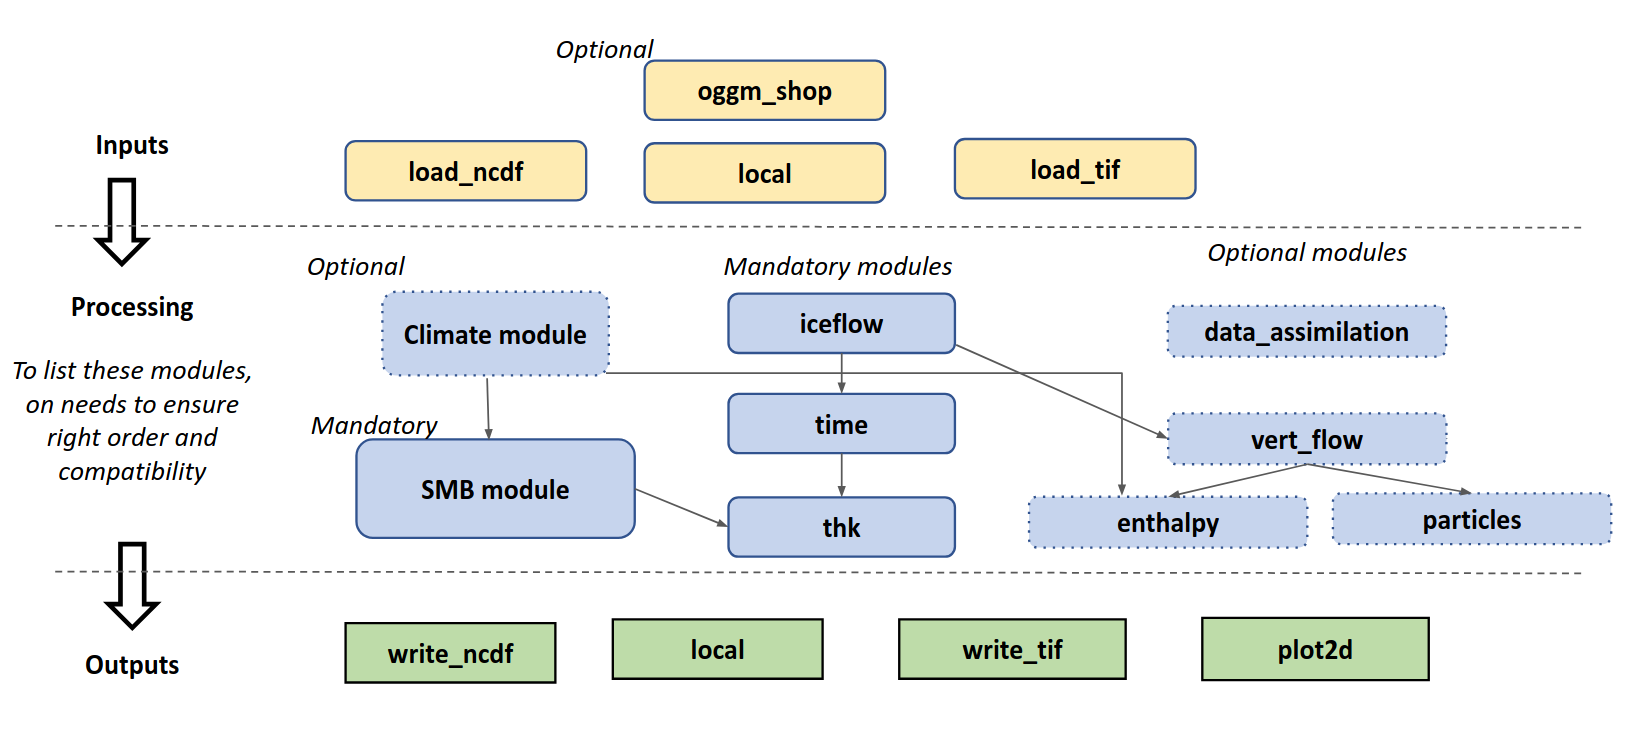
\includegraphics[width=\textwidth]{fig/flowchat-module.png}
\caption{Flowchart of IGM modules. }
\label{flowchart}
\end{center}
\end{figure*}

In the following sections, we give a brief description of the most important IGM modules, each identified by a keyword, and we refer to the documentation (\url{https://instructed-glacier-model.github.io/igm-doc/}) of each module for more details.

\subsection{Inputs modules}

IGM comes with input modules that can collect them from a database (\texttt{oggm\_shop}) and/or read raster data from files (\texttt{local}), 

Module \texttt{local} were built to load spatial 2D raster data from a NetCDF or Tiff file in IGM. The module is expected to import at least the basal topography, which is represented by variable \texttt{topg}, but can provide other fields such as the initial ice thickness \texttt{thk} and more. IGM has naming convention that must be followed to be recognized. Any field present in the NetCDF file will be passed and be available in IGM. At this stage, raster data can be resampled, coarsened or cropped to a specific regions.

Module \texttt{oggm\_shop} utilizes the Open Glacier Global Model \citep[OGGM][]{maussion2019open} (and then depends on python package \texttt{oggm}) to acquire data for contemporary glaciers. Users provide the RGI ID of the glacier of interest(\url{https://www.glims.org/maps/glims}). The data provided by OGGM are either already processed for certain spatial resolution and margin size, otherwise can be re-processed on demand to obtain certain user-defined spatial resolutions and/or margin sizes. Upon running this module, its automatically downloads an ensemble of data related to the specified glacier, which is then stored in a folder named after the RGI ID in folder \texttt{data}. Users can select 2D gridded variables of interest from the available products of the \texttt{oggm\_shop} to be writen in a IGM-readable NetCDF file thanks to \texttt{local} module.

\subsection{Processes modules}

Processes modules implement update rules for all modelled variables within the time loop. Modules correspond to specific physical components. For instance, the \texttt{iceflow} module updates the ice velocity, the \texttt{thk} module updates the ice thickness, and so on. Processes modules are conveniently listed in order: for instance, \texttt{iceflow} must come before \texttt{thk} as the latter needs the first.

\subsubsection{Data assimilation}
\label{data_assimilation}

This module permits to carry the data assimilation (or inverse modelling) while ensuring the consistence with the ice flow physics (Section \ref{inv_model}). It can be activated as a preliminary step to a forward or prognostic model run that assumes isothermal ice (i.e. without additional \texttt{enthalpy} module, since the the thermal condition are inferred from the inversion rather than computed from the enthalpy module). Running this module requires that necessary observational data have been loading in IGM using an inputs module such as ice surface ice velocities ${\bf u}^{s,obs}$, the top surface elevation $s^{obs}$, some ice thickness profiles $h_p^{obs}$, observed flux divergence $d^{obs}$, glacier mask from RGI outlines. A formerly-inferred ice thickness field \citep{farinotti2019consensus,millan2022ice} can be used to initialize the inverse model. All the observational data (including individual ice thickness profiles) are rasterized on the same grid, with possible no-data (NaN) values that are ignored in the optimization. While the optimization problem is presented in its most general form (Section \ref{inv_model}), the user selects a sub-ensemble of controls and constraints within the cost function based on the availability of data. Maintaining a balance between controls and costs/constraints is crucial to maintaining the well-posedness of the problem and guarding against multiple solutions. There are a couple parameters that need adjustement including i) confidence levels (i.e. tolerance to fit the data) $\sigma^u, \sigma^h, \sigma^s, \sigma^d$ or ii) regularization weights $\alpha^h, \alpha^c, \alpha^A$. The data assimilation is monitored through the iterations thanks to misfit cost component. 

\subsubsection{Climate}
\label{module_climate}

Climate modules \texttt{clim\_XXX} implement climate forcing in IGM as required by the SMB or enthalpy models. They supply distributed field of near surface air temperature, and precipitation at a given time resolution (e.g. daily, weekly or monthly). Module \texttt{clim\_oggm} reads monthly time series of historical climate data collected by the \texttt{oggm\_shop} module, and generates monthly 2D raster fields of precipitation, mean temperature, and temperature variability extrapolated to the entire glacier surface using a reference height and a vertical lapse rates. Module \texttt{clim\_deltat} loads a climate snapshot (associated to a certain period) and superposes a time-varying temperature offset (climate signal) that is often taken from paleo cliamte proxies \citep{seguinot2018modelling}. Module \texttt{clim\_glacialindex} loads two climate snapshots (associated to a certain periods) and interpolate them using a climate signal and a glacial index approach \citep{jouvet2023coupled}.

\subsubsection{Surface mass balance}
\label{module_smb}

Surface mass balance (SMB) modules \texttt{smb\_XXX} provide a rule to update the SMB. Module \texttt{smb\_simple} implements the SMB model defined by \eqref{smb1}-\eqref{smb2}. To that aim, the four parameters $z_{ELA}$, $\beta_{abl}$, $\beta_{acc}$, $m_{acc}$ are provided in an array for some times, and the module interpolates linearly them to provide a continous-in-time parametrization of the SMB. Module \texttt{smb\_oggm} implements a monthly PDD model calibrated on geodetic mass balance data \citep{hugonnet2021accelerated} by OGGM \citep{maussion2019open}. The yearly SMB at any point is computed with \eqref{smb3} from monthly temperature and precipitation fields as described in Section \ref{module_climate}. Laslty, module \texttt{smb\_accmelt} implements the combined snow accumulation / PDD model with the tracking of the snow layer.
 
\subsubsection{Ice flow}
\label{module_iceflow}

Module \texttt{iceflow} permits to use and retrain the emulator to update the ice flow in the forward modle. The latter relies on the ice flow emulator, which delivers ice flow field computationally efficiently. The user must first define physical parameters related to the ice flow (unless those were optimized in the data assimilation step), as well as parameters related to the vertical discretization (e.g., the number of vertical layers). Two other numerical parameters may need adjustements: i) the learning rate for the retraining of the CNN, which controls the strengh of retraining, ii) the retraining frequency, which needs to be sufficiently frequent to maintain accuracy, but not too much to mitigate computational costs. When treating large arrays, retraining must be done sequentially patch-wise for memory reason. The maximum size of patches is controlled by a parameter, which can be adpated to the size of the GPU memory. Last, it is possible to use a solver (instead of an emulator) to compute the iceflow, as well as using both the emulator and the solver (in diagnostic mode) to assess the fidelity of the iceflow emulator to the solver.

\subsubsection{Time}
\label{module_time}

Module \texttt{time} computes the time step (and update the time) with the following criteria: i) it is adjusted precisely to allow matching with specified saving times, whose the frequency is user-defined, ii) it remains below a designated maximum time step (often taken to one year to ensure that the time step is never too large), iii) it complies to the CFL condition \eqref{cfl}, which ensures stability in the transport scheme for ice thickness evolution. The simulation starting and ending time parameters are part of this module.

\subsubsection{Ice thickness}
\label{module_thk}

This module solves the mass conservation equation \eqref{conservationeq} using an explicit first-order upwind finite-volume scheme (as described in Section \ref{num_mass_conservation}). It permits to update ice thickness based on the results obtained from the \texttt{iceflow} and \texttt{smb\_XXX} modules. 

\subsubsection{Vertical ice flow}
\label{module_vertical}

Since the \texttt{iceflow} module is based on the Blatter-Pattyn ice flow model and predicts only the horizontal components of ice velocity, an additional module, \texttt{vert\_flow} additionally computes the vertical component by integrating the incompressibility condition \eqref{eq_incomp}. Module \texttt{vert\_flow} module is mandatory in various other modules, such as the \texttt{particle} and the \texttt{enthalpy} module.

\subsubsection{Enthalpy}
\label{module_enthalpy}

Module \texttt{enthalpy} permits to update the 3D fields enthalpy (or equivalently the temperature and water content), and the 2D water thickness in the till given these quantities at previous time step, as well the 3D iceflow following the numerical scheme described in Section \ref{module_enthalpy}. In turn, this permits to update the sliding coefficient as well as the Arrhenius factor, which are used in the \texttt{iceflow} module.
\subsubsection{Particles}
\label{module_particles}

Module \texttt{particles} permits to seed and track the position of virtual particles advected by the ice flow following the two methods described in Section \ref{num_particle_tracking}. By default, the module seeds the accumulation area at regular intervals, however, the seeding can be easily customized.

\subsection{Outputs modules}

Outputs modules permit to monitor the results of IGM. The frequency of saving is determined by a parameter defined within the \texttt{time} module (as this time needs to be reached exactly). Module \texttt{local} are responsible for writing 2D field variables that are specified in the parameter lists in NetCDF or Tif format files. Module \texttt{plot2d} module generates 2D plan-view plots of user-defined variables, which can be displayed in real-time or saved as image files. 

\subsection{User modules}
\label{user_modules}

Beside the modules listed above, IGM users can write their own inputs, processes, or outputs modules to load differently the data, couple new processes, or output the results in a different format. For each processes module, the user must provide three functions that are called at initialization, during the time loop, and at the end: \texttt{initialize(cfg,state)}, \texttt{update(cfg,state)}, and \texttt{finalize(cfg,state)}, while only one function \texttt{rune(cfg,state)} is required for inputs and outputs modules.  Herabove, \texttt{cfg} contains all the parameters needed for the simulation, organized by attributes in a hierachical manner. They include "core" parameters (independant to any modules), and module-related ones (e.g., \texttt{cgf.processes.time.start} is the initial simulation time). On the other hand, \texttt{state} holds all the variables at a specific time (e.g., \texttt{state.U} and \texttt{state.thk} denotes the 3D ice flow and the 2D ice thickness fields). These variables are updated throughout the simulation to represent the evolving state of the glacier.

\section{Applications} 

\textcolor{red}{[TO COMPLETE]} 

%\subsection{ISMIP-HOM experiments}

%\textcolor{red}{[GJ: TODO, see \citep{jouvet2023ice}]} 

\subsection{Enthalpy experiments}

\textcolor{red}{[GJ: TOCHECK]} 

Following \citep{wang2020two}, we carry the two benchmark experiments proposed by 
\citep{kleiner2015enthalpy} and one from \citep{hewitt2017models} to
verify the implementation of the enthalpy formulation.

Experiment A considers a flat parallel-sided slab with a constant thickness $h$ = 1000 m
without any ice dynamics so that only the vertical heat diffusion is modelled. We perform
a transient simulation during 300'000 years with a constant geothermal heat flux at the base. 
The surface temperatures are prescribed to -30$^{\circ}$C all the time except between
$t=100'000$ years and $t=150'000$ years. Fig. \ref{KleinerExpA} 
shows the time series of the simulated basal temperatures,
basal melt rates, and basal water layer thicknesses. As a result, they compare very well with 
with reference solutions shown in Fig 1 of \citep{kleiner2015enthalpy}. 

\begin{figure}[!h]
\begin{center} 
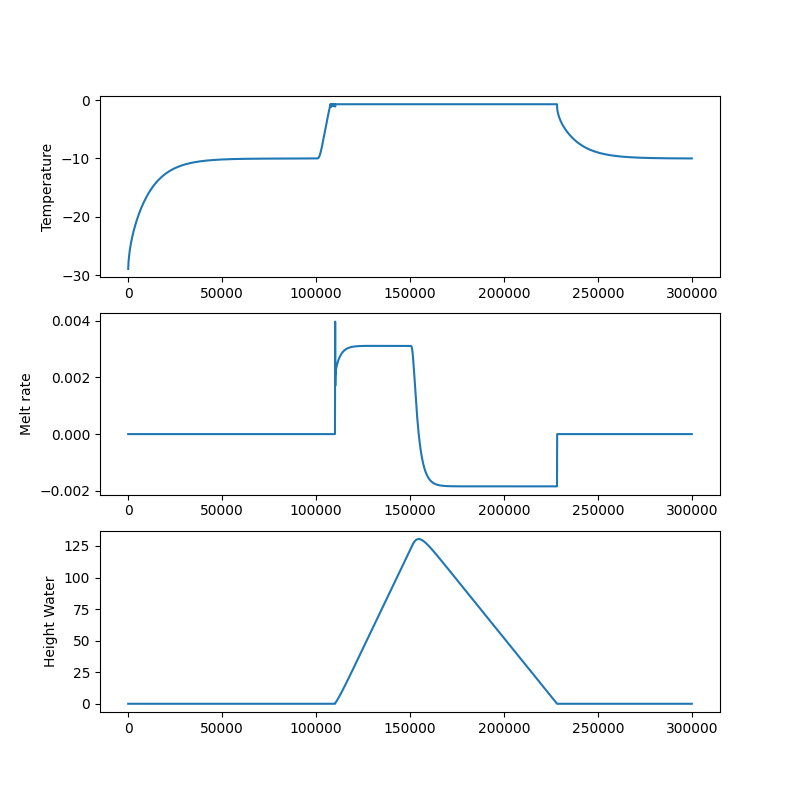
\includegraphics[width=0.48\textwidth]{fig/KleinerExpA.png}   
\end{center}
\caption{ Result of experiment A of \citep{kleiner2015enthalpy}. \label{KleinerExpA}}
\end{figure}

Experiment B also considers a parallel-sided slab but with a constant thickness $h=200$ m
and a slope of 4 $^{\circ}$. The horizontal ice velocity is defined by a SIA-like profile, 
while the vertical ice velocity is constant. 
The enthalpy at the surface is prescribed with -3$^{\circ}$C and zero water content.
We assume zero geothermal heat flux and basal sliding velocity.
Here, only the strain heating acts as heat source. We initialize 
the transient simulation with a constant enthalpy field with -1.5$^{\circ}$C 
and zero water content. We assume the thermal diffusivity of temperate ice to be 
100'000 times lower than the one of the cold ice. We run the simulation until
reaching a steady state, which is after 1000 years.
As a result, they compare well with 
the reference solution shown in Fig 4 of \citep{kleiner2015enthalpy}. 

\begin{figure}[!h]
\begin{center} 
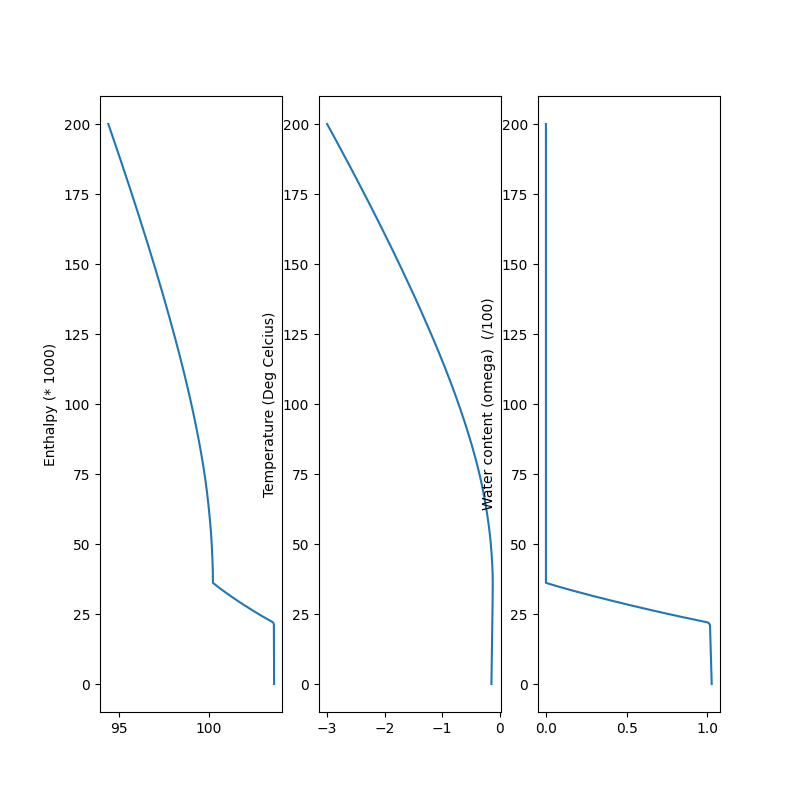
\includegraphics[width=0.48\textwidth]{fig/KleinerExpB.png}   
\end{center}
\caption{ Result of experiment B of \citep{kleiner2015enthalpy}. \label{KleinerExpB}}
\end{figure}

Last, we reproduced the experiment proposed by \citet{hewitt2017models},
which consider an idealized ice cap geometry. Again, the horizontal ice velocity 
and the strain heating are defined based on SIA-like ice flow. We impose 
a constant temperature on the top surface of the ice cap, while we assume 
the bedrock to be at the pressure melting point. The simulation is initialized 
with a constant enthalpy field  with -11$^{\circ}$C and zero water content.
The simulation is run until steady state.
Fig. \eqref{hewitt2017} shows the result at steady-state with a drainage function.
As a result, it compares reasonably with the reference solution shown in Fig 7b 
of \citep{hewitt2017models}. It is likely that a higher number of layers would
imporve the match between the two.

\begin{figure}[!h]
\begin{center} 
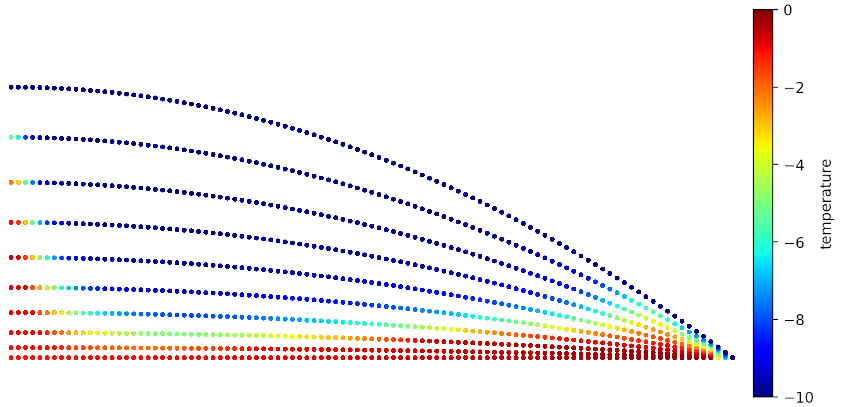
\includegraphics[width=0.48\textwidth]{fig/hewitt2017.png}   
\end{center}
\caption{ Result of the ice cap experiment  of \citep{hewitt2017models}. \label{hewitt2017}}
\end{figure}


%\subsection{Fidelity emulator / solver}

%\textcolor{red}{[GJ: TODO]} 

%\subsection{Inversion results}

%\textcolor{red}{[GJ: TODO]} 

%\subsection{particle tracking}

%\textcolor{red}{[GJ: TODO]} 

%\subsection{paleo / large array}

%\textcolor{red}{[GJ: TODO]} 

\conclusions  %% \conclusions[modified heading if necessary]
TEXT

%% The following commands are for the statements about the availability of data sets and/or software code corresponding to the manuscript.
%% It is strongly recommended to make use of these sections in case data sets and/or software code have been part of your research the article is based on.

\codeavailability{TEXT} %% use this section when having only software code available


\dataavailability{TEXT} %% use this section when having only data sets available


\codedataavailability{TEXT} %% use this section when having data sets and software code available


\sampleavailability{TEXT} %% use this section when having geoscientific samples available


\videosupplement{TEXT} %% use this section when having video supplements available


\appendix
\section{}    %% Appendix A

\subsection{}     %% Appendix A1, A2, etc.


\noappendix       %% use this to mark the end of the appendix section. Otherwise the figures might be numbered incorrectly (e.g. 10 instead of 1).

%% Regarding figures and tables in appendices, the following two options are possible depending on your general handling of figures and tables in the manuscript environment:

%% Option 1: If you sorted all figures and tables into the sections of the text, please also sort the appendix figures and appendix tables into the respective appendix sections.
%% They will be correctly named automatically.

%% Option 2: If you put all figures after the reference list, please insert appendix tables and figures after the normal tables and figures.
%% To rename them correctly to A1, A2, etc., please add the following commands in front of them:

\appendixfigures  %% needs to be added in front of appendix figures

\appendixtables   %% needs to be added in front of appendix tables

%% Please add \clearpage between each table and/or figure. Further guidelines on figures and tables can be found below.



\authorcontribution{TEXT} %% this section is mandatory

\competinginterests{TEXT} %% this section is mandatory even if you declare that no competing interests are present

\disclaimer{TEXT} %% optional section

\begin{acknowledgements}
TEXT
\end{acknowledgements}

%% REFERENCES
\bibliographystyle{copernicus}
\bibliography{biblio}



%% Since the Copernicus LaTeX package includes the BibTeX style file copernicus.bst,
%% authors experienced with BibTeX only have to include the following two lines:
%%
%% \bibliographystyle{copernicus}
%% \bibliography{example.bib}
%%
%% URLs and DOIs can be entered in your BibTeX file as:
%%
%% URL = {http://www.xyz.org/~jones/idx_g.htm}
%% DOI = {10.5194/xyz}


%% LITERATURE CITATIONS
%%
%% command                        & example result
%% \citet{jones90}|               & Jones et al. (1990)
%% \citep{jones90}|               & (Jones et al., 1990)
%% \citep{jones90,jones93}|       & (Jones et al., 1990, 1993)
%% \citep[p.~32]{jones90}|        & (Jones et al., 1990, p.~32)
%% \citep[e.g.,][]{jones90}|      & (e.g., Jones et al., 1990)
%% \citep[e.g.,][p.~32]{jones90}| & (e.g., Jones et al., 1990, p.~32)
%% \citeauthor{jones90}|          & Jones et al.
%% \citeyear{jones90}|            & 1990



%% FIGURES

%% When figures and tables are placed at the end of the MS (article in one-column style), please add \clearpage
%% between bibliography and first table and/or figure as well as between each table and/or figure.

% The figure files should be labelled correctly with Arabic numerals (e.g. fig01.jpg, fig02.png).


%% ONE-COLUMN FIGURES

%%f
%\begin{figure}[t]
%\includegraphics[width=8.3cm]{FILE NAME}
%\caption{TEXT}
%\end{figure}
%
%%% TWO-COLUMN FIGURES
%
%%f
%\begin{figure*}[t]
%\includegraphics[width=12cm]{FILE NAME}
%\caption{TEXT}
%\end{figure*}
%
%
%%% TABLES
%%%
%%% The different columns must be seperated with a & command and should
%%% end with \\ to identify the column brake.
%
%%% ONE-COLUMN TABLE
%
%%t
%\begin{table}[t]
%\caption{TEXT}
%\begin{tabular}{column = lcr}
%\tophline
%
%\middlehline
%
%\bottomhline
%\end{tabular}
%\belowtable{} % Table Footnotes
%\end{table}
%
%%% TWO-COLUMN TABLE
%
%%t
%\begin{table*}[t]
%\caption{TEXT}
%\begin{tabular}{column = lcr}
%\tophline
%
%\middlehline
%
%\bottomhline
%\end{tabular}
%\belowtable{} % Table Footnotes
%\end{table*}
%
%%% LANDSCAPE TABLE
%
%%t
%\begin{sidewaystable*}[t]
%\caption{TEXT}
%\begin{tabular}{column = lcr}
%\tophline
%
%\middlehline
%
%\bottomhline
%\end{tabular}
%\belowtable{} % Table Footnotes
%\end{sidewaystable*}
%
%
%%% MATHEMATICAL EXPRESSIONS
%
%%% All papers typeset by Copernicus Publications follow the math typesetting regulations
%%% given by the IUPAC Green Book (IUPAC: Quantities, Units and Symbols in Physical Chemistry,
%%% 2nd Edn., Blackwell Science, available at: http://old.iupac.org/publications/books/gbook/green_book_2ed.pdf, 1993).
%%%
%%% Physical quantities/variables are typeset in italic font (t for time, T for Temperature)
%%% Indices which are not defined are typeset in italic font (x, y, z, a, b, c)
%%% Items/objects which are defined are typeset in roman font (Car A, Car B)
%%% Descriptions/specifications which are defined by itself are typeset in roman font (abs, rel, ref, tot, net, ice)
%%% Abbreviations from 2 letters are typeset in roman font (RH, LAI)
%%% Vectors are identified in bold italic font using \vec{x}
%%% Matrices are identified in bold roman font
%%% Multiplication signs are typeset using the LaTeX commands \times (for vector products, grids, and exponential notations) or \cdot
%%% The character * should not be applied as mutliplication sign
%
%
%%% EQUATIONS
%
%%% Single-row equation
%
%\begin{equation}
%
%\end{equation}
%
%%% Multiline equation
%
%\begin{align}
%& 3 + 5 = 8\\
%& 3 + 5 = 8\\
%& 3 + 5 = 8
%\end{align}
%
%
%%% MATRICES
%
%\begin{matrix}
%x & y & z\\
%x & y & z\\
%x & y & z\\
%\end{matrix}
%
%
%%% ALGORITHM
%
%\begin{algorithm}
%\caption{...}
%\label{a1}
%\begin{algorithmic}
%...
%\end{algorithmic}
%\end{algorithm}
%
%
%%% CHEMICAL FORMULAS AND REACTIONS
%
%%% For formulas embedded in the text, please use \chem{}
%
%%% The reaction environment creates labels including the letter R, i.e. (R1), (R2), etc.
%
%\begin{reaction}
%%% \rightarrow should be used for normal (one-way) chemical reactions
%%% \rightleftharpoons should be used for equilibria
%%% \leftrightarrow should be used for resonance structures
%\end{reaction}
%
%
%%% PHYSICAL UNITS
%%%
%%% Please use \unit{} and apply the exponential notation


\end{document}
